% File project.tex
%% Style files for ACL 2021
\documentclass[11pt,a4paper]{article}
\usepackage[hyperref]{acl2021}
\usepackage{times}
\usepackage{booktabs}
\usepackage[draft]{todonotes}
\usepackage{latexsym}
% \usepackage[demo]{graphicx}
\usepackage{subcaption}
\usepackage[title]{appendix}
\usepackage{float}
\usepackage{amsmath}
\usepackage{indentfirst}
\usepackage{xcolor}
\usepackage{natbib}


% \usepackage{subfig}
\renewcommand{\UrlFont}{\ttfamily\small}


% Packages for collaborative annotations
\usepackage{comment}
%\usepackage[draft]{todonotes}
% This is not strictly necessary, and may be commented out,
% but it will improve the layout of the manuscript,
% and will typically save some space.
\usepackage{microtype}

\aclfinalcopy 

\newcommand\BibTeX{B\textsc{ib}\TeX}

\title{11-777 Spring 2021 Class Project}

\author{
  Yun Cheng\thanks{\hspace{4pt}Everyone Contributed Equally -- Alphabetical order} \hspace{2em} Yuxuan Liu$^*$ \hspace{2em} Tiffany Ma$^*$ \hspace{2em} Erin Zhang$^*$ \\
  \texttt{\{yuncheng, yuxuanli, tma1, xiaoyuz1\}@andrew.cmu.edu}
}

\date{\today}

\begin{document}
\maketitle
\begin{abstract}
Template for 11-777 Reports using the ACL 2021 Style File 
\end{abstract}

\section{Introduction and Problem Definition}

% \begin{figure}
% \missingfigure[figwidth=\linewidth]{This is a simple example/demonstration figure that explains your task and insight}
% \end{figure}

\clearpage
\newcommand{\red}[1]{{\color{red}{#1}}}


\section{Related Work and Background}
\paragraph{Action segmentation} The goal of action segmentation is to temporarily localize action segments and classify the category of the action in each segment in an untrimmed input video. The application of action segmentation can be found in various fields such as robotics \cite{robotics_action_seg} and behavior analysis \cite{shao2012human}. Action segmentation is closely related but different from action recognition and action detection. Action recognition identifies one action in a trimmed video, and action detection usually outputs a sparse set of actions. By contrast, action segmentation is a more complex task that considers a longer range of temporal relations between sequential activities for more fine-grained action recognition in an untrimmed video.

\paragraph{Early works}
Traditional approaches generally fall into three categories: sliding window approaches, segmental models, and recurrent networks \cite{graphbased2020}. One of the earliest attempts is to detect action segments with temporal windows of different scales and non-maximum suppression \cite{6247801}. However, this method is limited by the tradeoff between larger window size and computational costs. Others use segmental models like spatiotemporal CNNs with the semi-Markov model for tracking object relationships, action transitions, and environment change \cite{lea2016segmental, 6619177}. With each action conditioned on the previous one, these methods are good at capturing local dependencies in consecutive visual patterns rather than long-range temporal relations. Other hybrid approaches include representing frames using Fisher Vectors with HMMs and GRUs for temporal modeling \cite{7477701, 8099623}, which have their main drawback of efficiency. Another line of research focuses on temporal convolutional networks (TCNs) that perform fine-grained action segmentation using temporal convolutions \cite{lea2016temporal}. The method is extended to a multi-stage architecture with a set of dilated temporal
convolutions in each stage. It is proven to be able to avoid temporal pooling and better capture long-range dependencies \cite{farha2019mstcn}.  

\paragraph{Graph convolution networks} Recently, existing models are further improved by the introduction of graph convolution networks (GCNs). Built on top of action segmentation models, the graph-based module models the temporal relations between initial segmentation results with temporal proximity. It refines the pre-computed action segments by performing segment boundary regression and segment classification \cite{graphbased2020}. The latest extension to this approach constructs multi-level dilated temporal graphs for temporal reasoning at different timescales \cite{wang2020temporal}. The limitations of the graph-based module exist in its dependence on the initial backbone output. For example, it suffers from low efficiency on large graphs if the initial segmentation is heavily fragmented. However, while abundant works have been done in unimodal action segmentation, we observe that almost none of the existing work attempts at multimodal approaches. Since textual data is one of the most common and accessible annotations of video data, we are interested in incorporating texts as a complimentary domain for better segmentation results.

\paragraph{Text Alignment}
\iffalse
Covered paper:
- Multimodal Machine Learning: A Survey and Taxonomy
- Learning Semantic Concepts and Temporal Alignment for Narrated Video Procedural Captioning
- Unsupervised Learning from Narrated Instruction Videos
- What’s Cookin’? Interpreting Cooking Videos using Text, Speech and Vision
\fi
Identifying the relationship between two or more modalities is one of the core challenges in Multimodal settings \cite{MultiModalSurvey}. An example of unsupervised approaches to text alignment is to first perform temporal clustering individually on the video input and the text input, then use the two clusters to provide complementary information to one another \cite{unsupervised-align}. For instance, differences in two video segments can provide a temporal cue to a breaking point within the narrative script. Contextual information is used to assist the alignment of textual scripts and video frames \cite{temporalAlignShi}. It is built by firstly collecting a mean pooling of each modality within $K$ units. The mean representation of two modalities is then combined through a transformer model and concatenated to the embedding of the individual. Our task concerns video and scripts in the cooking domain. In one of the similar experiments, the text script is parsed into action-object (i.e. verb-noun) classes, and the video frames are aligned to the text script by matching the tokens of action-objects to those present in the frames \cite{malmaud-etal-2015-whats}.

\paragraph{Text-Image Matching}
To build better representation for the graph nodes, we want to use the narrations to attend to regions in the frame that are closely associated with the action that is conducted. In this way, different relevant objects in different frames can be used to distinguish the segment boundaries. 

To use attention methods, we first need to provide a set of image features. To better extract object features in the images, Faster R-CNN \cite{ren2016faster} firstly generates Region Of Interests (ROIs) with high objectness, and it then uses intermediate convolution feature maps to classify the region and regress bounding boxes. Fully Convolutional One-Stage Object Detection (FCOS) \cite{tian2019fcos} belongs to a family of anchor-less methods. Instead of regressing bounding boxes using the anchors as references, it regresses four values, $l,t,r,b$ that represent the distance from a location in the image to the four sides of the bounding boxes. Moreover, it uses CNN feature maps from different levels to perform bounding box regression at various scales to capture objects with different sizes. It has been shown that anchor-less detectors perform better than anchor-based detectors on seen and unseen test sets, and FCOS can identify objects involved in the action \cite{yoon2020semisupervised}.  

Given a set of image features, encoding regions in the image, and a set of word features extracted from the sentence, Stacked Cross Attention \cite{lee2018stacked} determines the similarity between image-sentence pair by inferring how important a region is to the sentence, and it can also reversely infer how important a sentence is to the image. An additional position feature is concatenated for the object with the visual feature extracted by ResNet \cite{wang2019position}. The image is divided into blocks, and embedding vectors representing the positions of the blocks are combined with weights determined by overlap between the block and the visual feature. The addition is motivated by the fact that the positions of objects in the image are related to the semantics of the image. This intuition aligns with our task since we expect that the relative positions of objects are associated with the action during cooking.

\clearpage

\section{Task Setup and Data (1 page)}
The main task is to segment egocentric (first-person) cooking videos from EPIC-KITCHENS dataset into action-object pairs. Given a video clip in the form of a sequence of frames, we want to identify the type of actions as well as their start and end time in the given video.


\subsection{Dataset}
% left out the word extended because we never mentioned EPIC-KITCHEN-55 %
We use the largest egocentric (first-person) dataset  EPIC-KITCHENS-100, which features 100 hours, 700 variable-length videos with 90K actions of 37 participants \cite{Damen2020RESCALING}. Compared to YouTube-based datasets such as HowTo100M \cite{miech19howto100m}, EPIC-KITCHENS contains activities that are non-scripted and thus capture more natural settings such as parallel tasking . The egocentric view provides a unique perspective on people-object interactions, attention, and intention. Meanwhile, it also imposes extra challenges compared to third-person datasets like YouCook2 \cite{ZhXuCoAAAI18}. One of the challenges is that certain actions, such as eating and drinking, cannot be directly observed due to the limited field of view. Other challenges include unseen participants, unseen cooking actions, frame noises from different sources (i.e. background and lighting), long videos with many action instances, fragmentation of segments resulted from interleaving actions in multi-tasking, and weaker temporal correlations in objects interfering the correlations in actions.

\subsection{Task formulation}
There are two input modalities: video frames of egocentric cooking scenes and narrations describing the action in the scenes. The narrations are transcribed from the audio in the form of imperative phrases: verb-noun with optional propositional phrase. The goal is to predict a verb class as well as a noun class for each frame to identify the action in the segments. Afterwards, we combine the two classes into a tuple as the final output class label. 

Formally, the visual input consists of a sequence of $M$ RGB frames in temporal order, denoted as $F=(\mathbf{f}_i)_{i=1}^M$. The RGB frames are sampled from untrimmed videos at a rate of 50 frames per second. The textual input is a sequence of $N$ audio-transcribed narrations in temporal order, denoted as $C=(\mathbf{c}_i)_{i=1}^N$. Our goal is to infer the action-object class label for each frame. The ground truth is given by $Y=(\mathbf{y}_i)_{i=1}^M$. Each $\mathbf{y}_i\in\{0,1\}^K\times\{0,1\}^L$ is a tuple of one-hot vectors encoding the true verb and noun class, where $K$ is the number of verb classes and $L$ is the number of noun classes.


\subsection{Dataset Statistics}

\subsubsection{Text Analysis}
Narrations in EPIC-KITCHENS-100 are mainly imperative phrases in the form of verb-noun with optional propositional phrase (e.g. \textit{put down plate}, \textit{put container on top of counter}). Each annotation includes start/stop frame indices. Action verbs and object nouns, which are extracted from the corresponding narration. Verbs and nouns are further classified into classes based on their semantic meaning. There are a total of 97 verb classes and 300 noun classes in the training and validation set.

We define the frequency of a verb/noun class as the number of narrations that contain a verb/noun from that class. Both verb and noun classes have a heavy tailed distribution with tail classes ($\le$ 1/15 of the maximum frequency) accounting for 13.02$\%$ and 11.67$\%$ total verbs and 5.38$\%$ and 1.85$\%$ total nouns in the training and validation set respectively (Figure \ref{fig:verb_freq}). Such a distribution indicates the intrinsic complexity and entropy of the text data. Since there were no constraints on the recording duration, we observe a great variability across videos. Average sentence length of training and validation set is 15.1 and 14.8 with standard deviation of 6.3 and 6.0 words, respectively. Average number of actions per video is 135.8 (training) and 70.1 (validation) with standard deviation of 167.7 and 93.2. More distribution statistics can be found in Appendix A Table \ref{table:train_val_stats}.

%A natural assumption of our task is that there is none or minimal overlapping between action segments, i.e. only one action in almost all time frames. We check that there are at most 4 narrations in parallel in training and 3 in validation; only 3832 (5.70$\%$) and 617 (0.92$\%$) pairs of consecutive actions overlap for more than 1 second. We also inspect the feature embeddings of the verb and noun classes. Using GloVe word vectors pre-trained on Twitter (200d vectors) \cite{pennington2014glove}, we do not notice significant interclass or intraclass clustering effect (Appendix \ref{appendix:A} Figure \ref{fig:embedding}).

% \begin{figure}[t!]
%     % \begin{minipage}[b]{1\textwidth}
%         \begin{subfigure}[b]{0.475\textwidth}
%             \centering
%             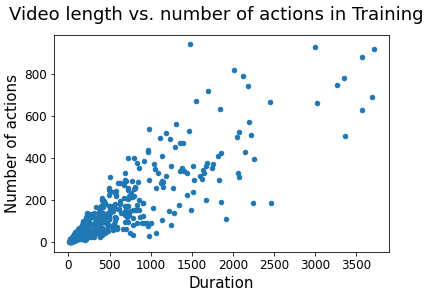
\includegraphics[scale=0.42]{figures/length_vs_actions_Training.png}
%         \end{subfigure}\\
%         \begin{subfigure}[b]{0.475\textwidth}
%             \centering
%             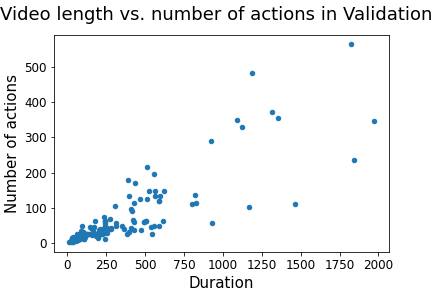
\includegraphics[scale=0.42]{figures/length_vs_actions_Validation.png}
%         \end{subfigure}
%         \caption{Number of action in each video against video length (in seconds)}
%         \label{fig:action-freq-video-length}
%     % \end{minipage}
% \end{figure}

\subsubsection{Video Frame Analysis}
We extract RGB frames from the videos at a sampling rate of 50 FPS. Each frame is identified by participant id, video id, and a start/end frame number. More than half of the total 700 videos in the dataset have less than 25,000 frames.  

Videos in EPIC-KITCHENS-100 have varied length with the longest video of 3708 seconds and shortest video of 10 seconds. 85.7 $\%$ of the videos are shorter than 1000 seconds and 66.0 $\%$ are less than 500 seconds (Appendix A Table \ref{table:train_val_stats}, Figure \ref{fig:duration}). 
%lacking sufficiency in support of longer videos.
% \cite{graphbased2020} mentioned that optimization tends to be slow for longer videos in action recognition tasks. 
We also see that the number of narrations grows roughly linearly with video length (Figure \ref{fig:action-freq-video-length}).  

%[Trim] If need to trim, we can trim on example words%
% The top-10 verb classes with the most number of frames include actions like \textit{grate, wait, prepare, knead, stir}, and \textit{cut}; while those with the least number of frames contain actions like \textit{bend, turn-off, turn-on, take, close}.  and the average length of the action aligns with how people would respond if asked about which action would take longer. It seems that actions involved during cooking take longer than those related to intermediate preparatory steps. 
We compile all training and validation samples of a given verb class and compute the average number of frames for this class (Appendix Figure \ref{fig:avg-frame}). For most verb classes, the average number of frames in each class are roughly the same in both training and validation set, except a few where the validation sets have more frames. We also count the total number of frames for each verb class, summed over all training and validation samples in the class. We notice that such frequency corresponds to the trend of verb-class frequency in the annotations (Appendix A Figure \ref{fig:total-frame}). This indicates that within the dataset, the frequency of the verb class correlates to the amount of visual information in the dataset.

%The dataset also provides bounding-box annotations for each frame, where it only distinguishes between two categories: hands and objects. Only active objects are annotated, so the number of object bounding-boxes in a frame approximates the number of objects that the person interacts with. We compute the average number of hand bounding-boxes appearing in a frame of each verb class. 
%Class with less than 1.5 hand bounding-boxes include actions like \textit{take, put-on, open, pull-down, walk}, and these correspond roughly to human impression on how many hands are needed for performing the action. We also compute the average number of objects bounding boxes in a frame of a given verb class. Verb classes with less than 1.8 object bounding boxes include actions like \textit{open, close, shake, check, fold}, and \textit{drink} (Appendix A Figure \ref{fig:hand-bbox}, \ref{fig:obj-bbox}). 
% \todo[inline]{Would be nice if we can generalize like more avg number of bounding boxes correlates to xx type of action?}
%The average numbers of hand and object bounding boxes for the training and validation sets are mostly equal, despite the validation set misses a few verb classes. Full details can be found in Appendix \ref{appendix:A}.




\subsection{Metrics}

\clearpage
\section{Models (2 pages)}

\subsection{Baselines}
Both existing baselines explained with citations and novel ones missing from the current literature

\subsection{Proposed Approach}

\clearpage
\begin{table*}[t]
\centering
\begin{tabular}{lrrrr}
\toprule
                            & \multicolumn{2}{c}{Dev} & \multicolumn{2}{c}{Test}\\
Methods                     & Accuracy $\uparrow$ & $L_2$ Error $\downarrow$ & Accuracy $\uparrow$ & $L_2$ Error $\downarrow$ \\
\midrule
Previous Approach 1 \cite{} & & & & \\
Previous Approach 2 \cite{} & & & & \\
Previous Approach 3 \cite{} & & & & \\
\midrule
Proposed Method             & & & & \\
\bottomrule
\end{tabular}
\end{table*}
\section{Results (1 page)}
The columns above are just examples that should be expanded to include all metrics and baselines.

\clearpage
\section{Analysis (2 pages)}
This section should include at least two to three plots
\subsection{Ablations and Their Implications}

\subsection{Qualitative Analysis and Examples}
This section should likely contain a table of examples demonstrating how the current approach succeeds/fails.

% Please use 
\bibliographystyle{acl_natbib}
\bibliography{references}

\clearpage

\begin{appendices}
\section{Data Analysis}
\label{appendix:A}
\begin{minipage}{1\textwidth}
    In this section, we present the full details of our data analysis.
\end{minipage}
\begin{table}[ht!]
\begin{minipage}{1\textwidth}
\begin{center}
{\small
\begin{tabular}{lrrrrrrrr}
\toprule
& \multicolumn{4}{c}{Training} & \multicolumn{4}{c}{Validation}\\
~ & Max. & Min. & Avg. & Std. & Max. & Min. & Avg. & Std. \\
\midrule
Verb class frequency & 14848 & 73 & 1314 & 2829 & 1937 & 71 & 191 & 398\\
Noun class frequency & 3617 & 178 & 724 & 655 & 430 & 25 & 108 & 92\\
Sentence length & 77 & 3 & 15.1 & 6.3 & 71 & 3 & 14.8 & 6.0\\
Actions per video & 940 & 1 & 136 & 168 & 564 & 3 & 70 & 93\\
Frames per verb class & 2129212 & 20165 & 225170 & 408408 & 407425 & 2702 & 42016 & 76950 \\
Video length & 3708 & 10 & 543 & 645 & 1969 & 11 & 344 & 377 \\
\bottomrule
\end{tabular}}
\caption{Statistics of EPIC-KITCHENS-100 training and validation set}
\label{table:train_val_stats}
\end{center}
\end{minipage}
\end{table}

\begin{figure}[hp]
    \begin{minipage}{1\textwidth}
    \centering
        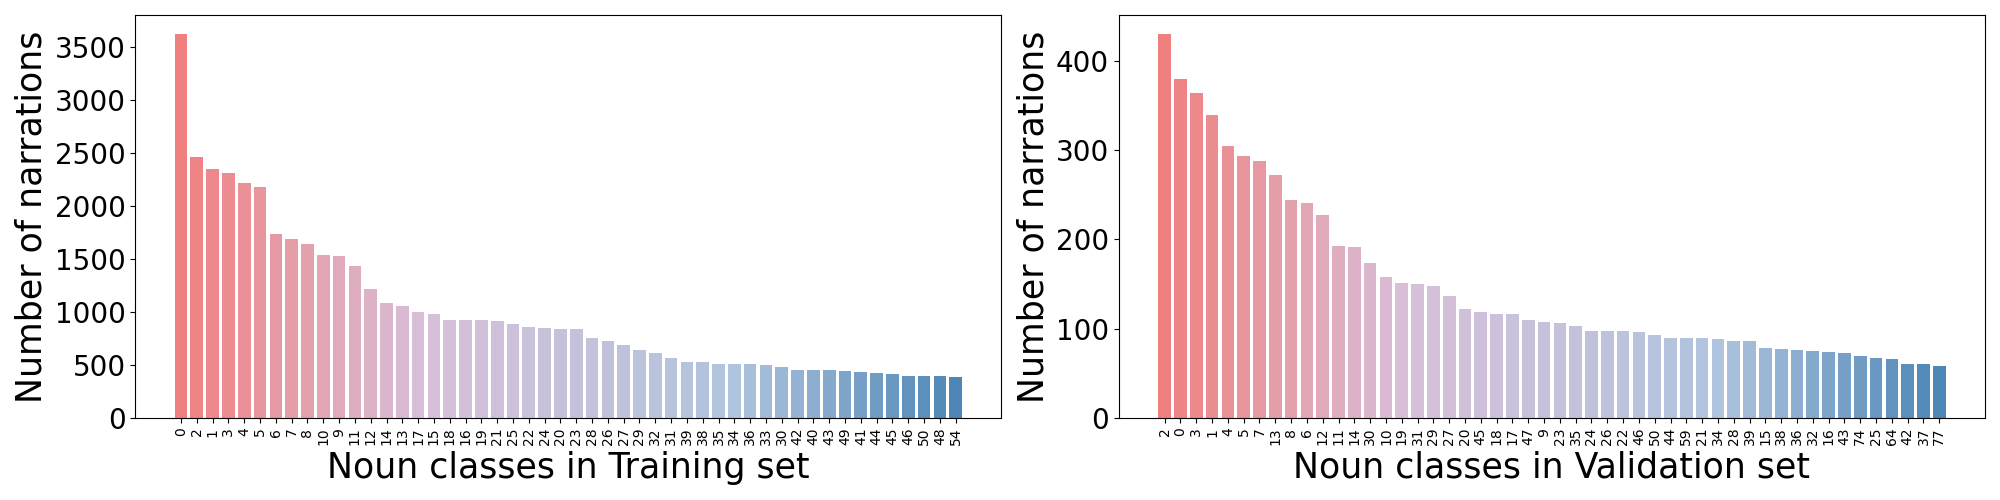
\includegraphics[scale=0.3]{figures/noun_count.png}
    \caption{Frequency distribution of 50 most frequent noun classes in training and validation set}
    \label{fig:noun-freq}
    \end{minipage}
\end{figure}
\begin{figure}[htp!]
    \begin{minipage}{1\textwidth}
        \begin{center}
            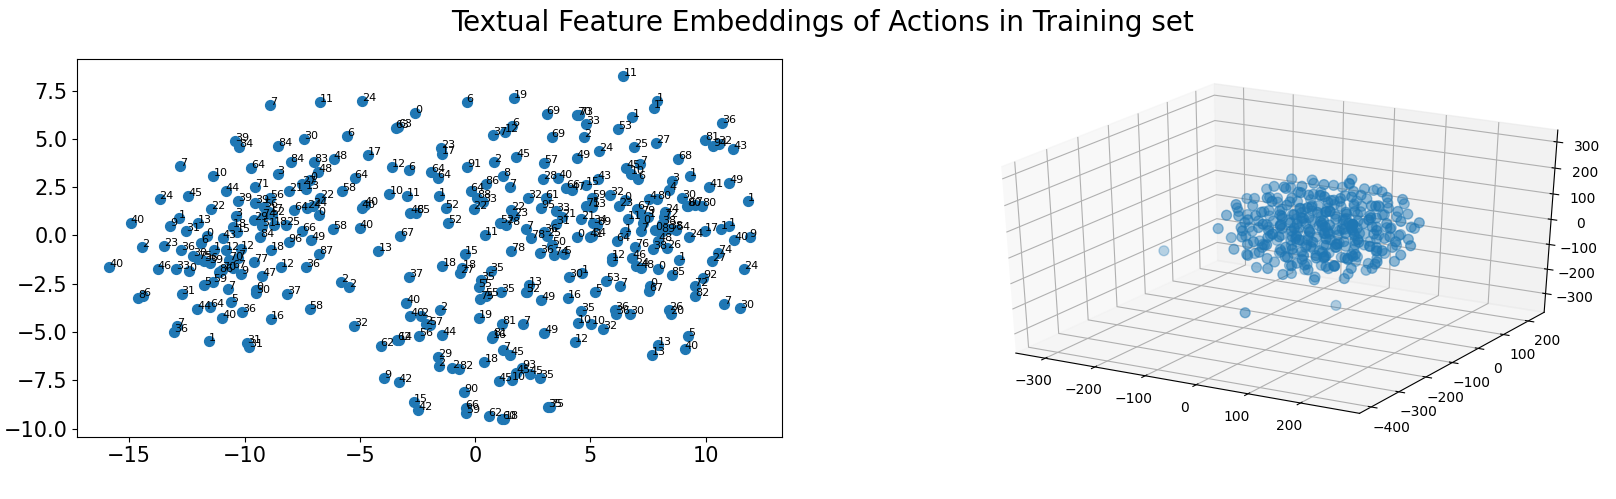
\includegraphics[scale=0.36]{figures/Actions_embeddings_Training.png}
            \\
            \vspace{5mm}
            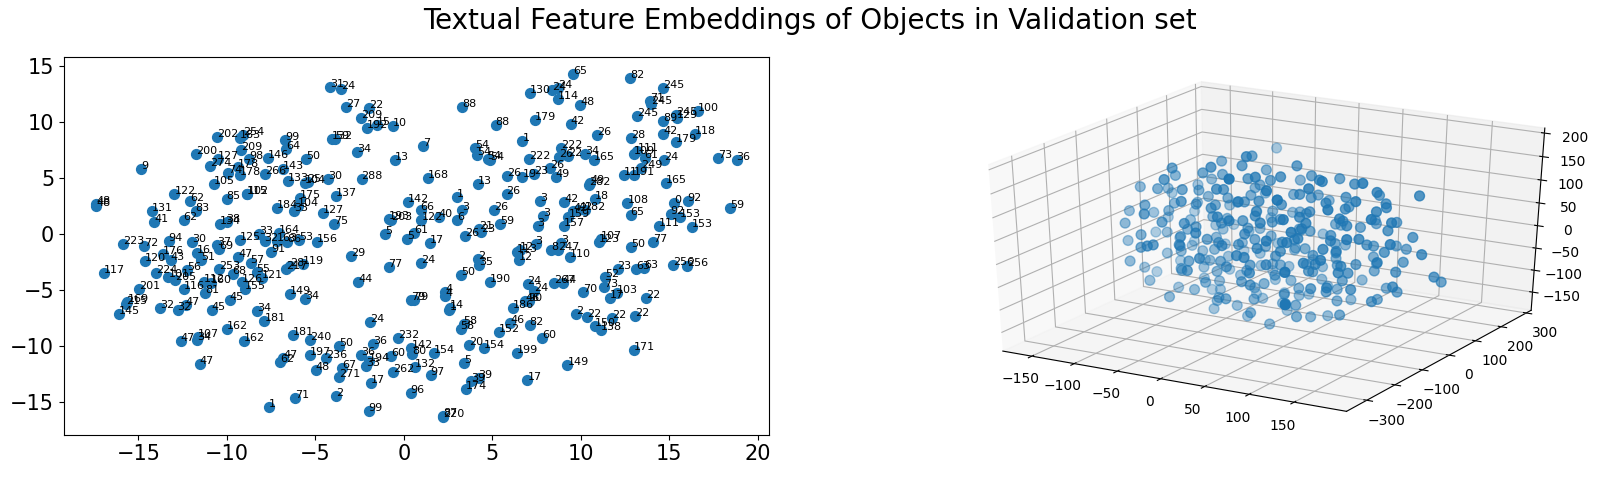
\includegraphics[scale=0.36]{figures/Objects_embeddings_Validation.png}
            \caption{Example of visualizing feature embeddings of verb and noun classes in 2D and 3D space}
            \label{fig:embedding}
        \end{center}
    \end{minipage}
\end{figure}
\clearpage

\begin{figure}[ht!]
    \begin{minipage}[b]{1\textwidth}
        \begin{subfigure}[b]{0.475\textwidth}
            \centering
            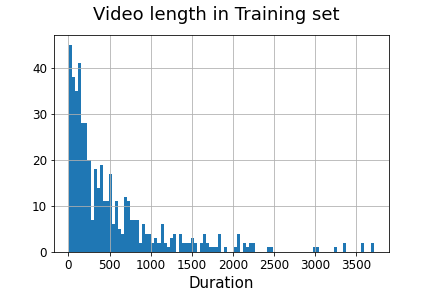
\includegraphics[scale=0.4]{figures/video_length_Training.png}
        \end{subfigure}
        \begin{subfigure}[b]{0.475\textwidth}
            \centering
            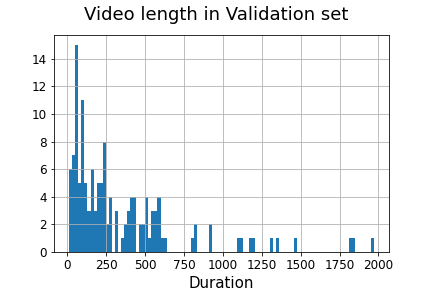
\includegraphics[scale=0.4]{figures/video_length_Validation.png}
        \end{subfigure}
        \caption{Distribution of video length (in seconds)}
        \label{fig:duration}
    \end{minipage}
\end{figure}

\begin{figure}[htp!]
    \begin{minipage}[b]{1\textwidth}
        \centering
        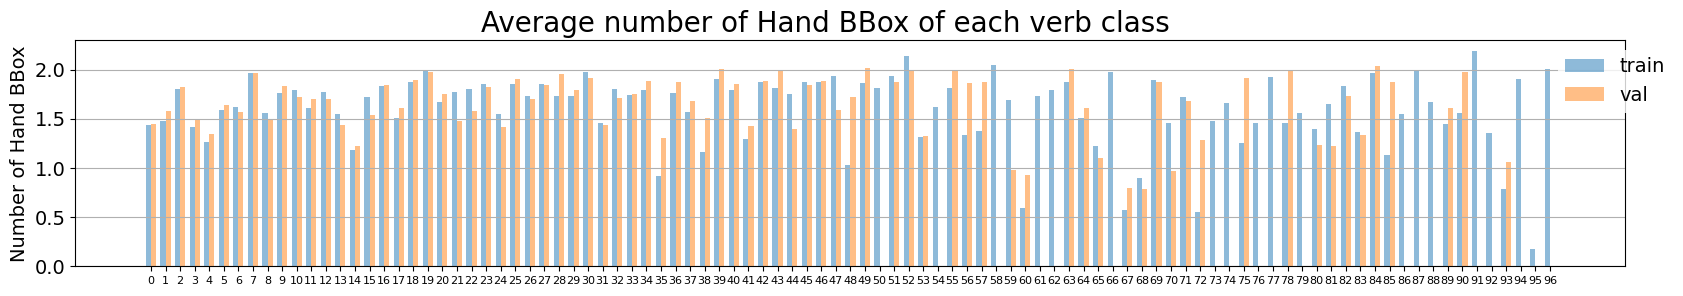
\includegraphics[scale=0.38]{figures/avg_number_Hand_bbox_verb_class.png}
        \caption{Average number of hand bounding-boxes in each frame of given verb class}
        \label{fig:hand-bbox}
    \end{minipage}
\end{figure}

\begin{figure}[htp!]
    \begin{minipage}[b]{1\textwidth}
        \centering
        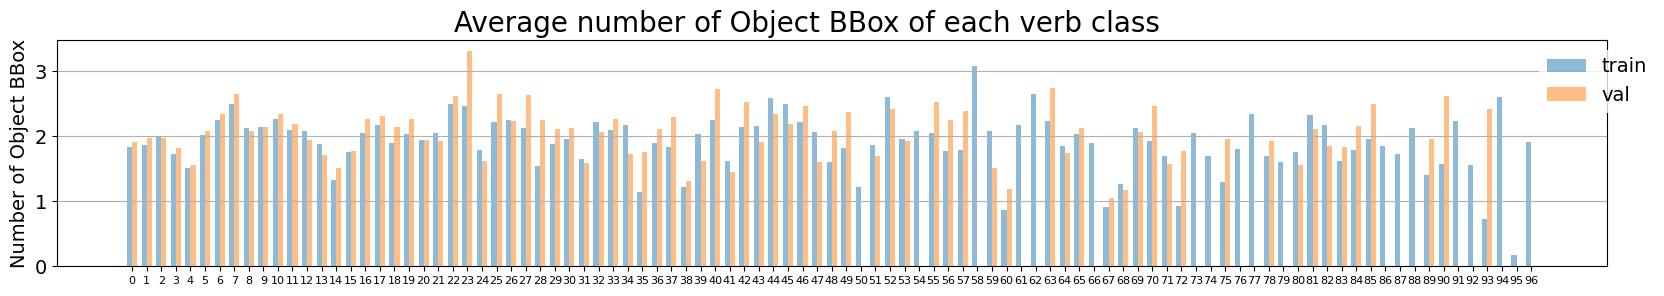
\includegraphics[scale=0.38]{figures/avg_number_Object_bbox_verb_class.png}
        \caption{Average number of object bounding-boxes in each frame of given verb class}
        \label{fig:obj-bbox}
    \end{minipage}
\end{figure}

\begin{figure}[htp!]
    \begin{minipage}[b]{1\textwidth}
        \centering
        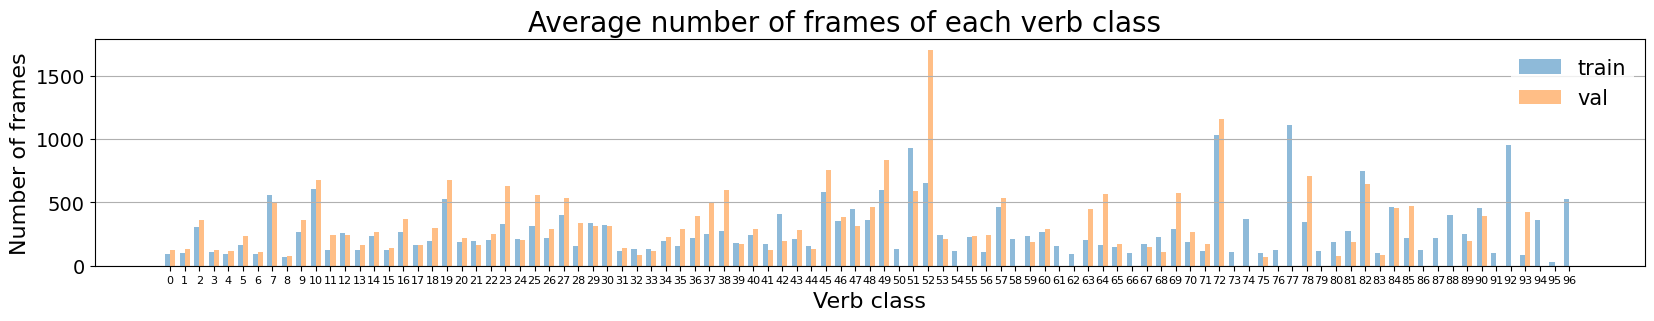
\includegraphics[scale=0.38]{figures/avg_number_frames_verb_class.png}
        \caption{Average number of frames in a narration of a given verb class in training and validation set}
        \label{fig:avg-frame}
    \end{minipage}
\end{figure}

% \begin{figure}[htp!]
% \begin{minipage}[b]{1\textwidth}
%     \begin{minipage}[b]{0.475\textwidth}
%         \begin{subfigure}[b]{0.475\textwidth}
%             \centering
%             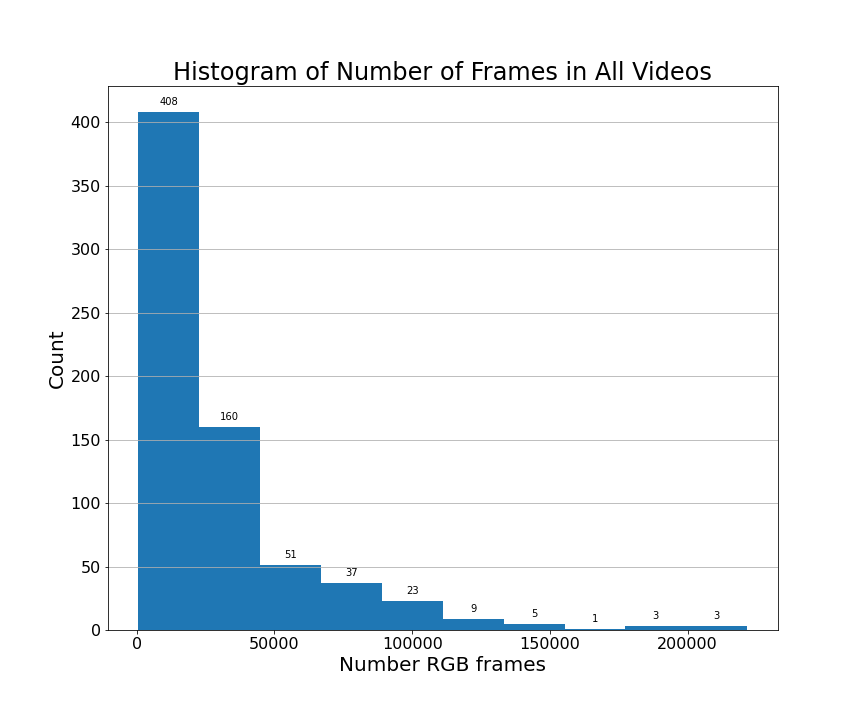
\includegraphics[scale=0.28]{figures/histogram_num_frame_videos.png}
        % \end{subfigure}
        % \begin{subfigure}[b]{0.475\textwidth}
        %     \centering
        %     \includegraphics[scale=0.3]{figures/avg_number_frames_verb_class_4.png}
        % \end{subfigure}
    %     \caption{Distribution of number of frames in each video}
    %     \label{fig:frame-video}
    % \end{minipage}
    % \hfill
    % \begin{minipage}[b]{0.475\textwidth}
    %     \begin{subfigure}[b]{0.475\textwidth}
    %         \centering
    %         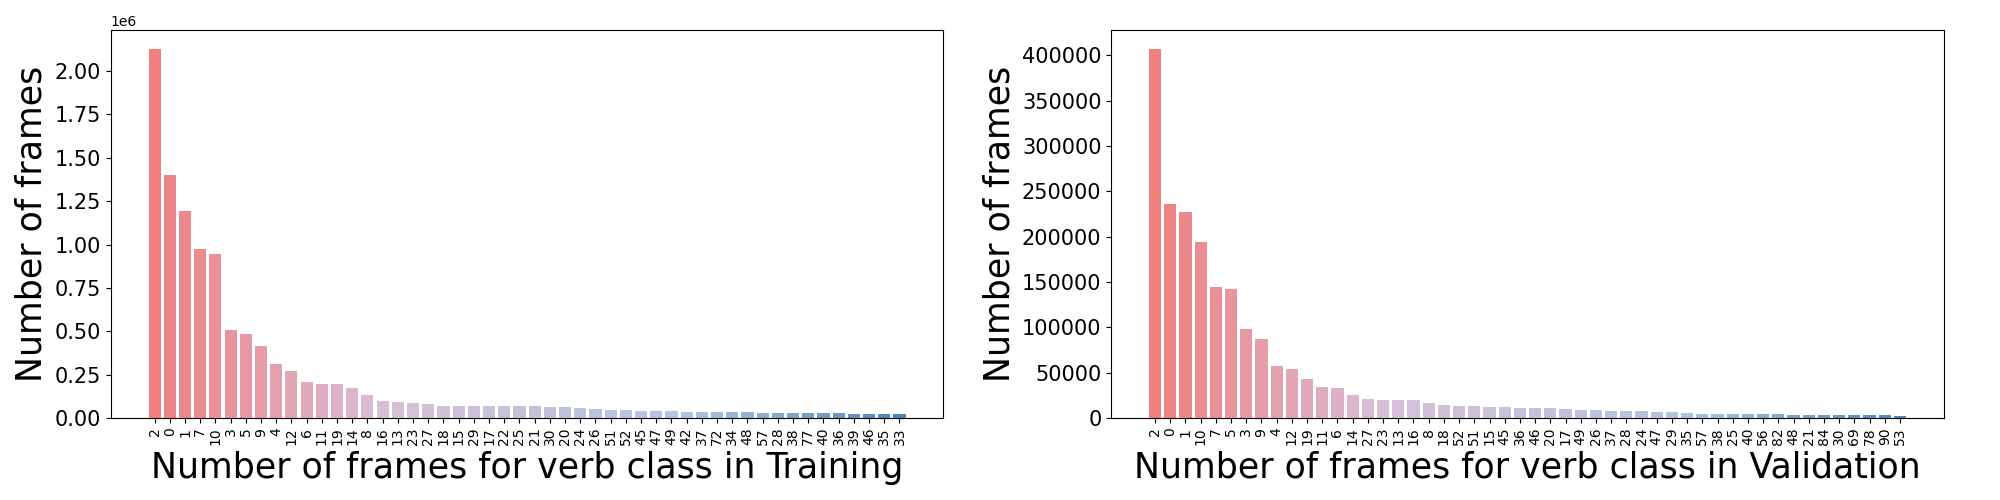
\includegraphics[scale=0.15]{figures/total_frame_word.png}
        % \end{subfigure}
        % \begin{subfigure}[b]{0.475\textwidth}
        %     \centering
        %     \includegraphics[scale=0.3]{figures/avg_number_frames_verb_class_4.png}
        % \end{subfigure}
%         \caption{Distribution of number of frames in each video}
%         \label{fig:total-frame}
%     \end{minipage}
% \end{minipage}
% \end{figure}

% \begin{figure}[htp!]
%     \begin{minipage}[b]{1\textwidth}
%         \begin{subfigure}[b]{0.475\textwidth}
%             \centering
%             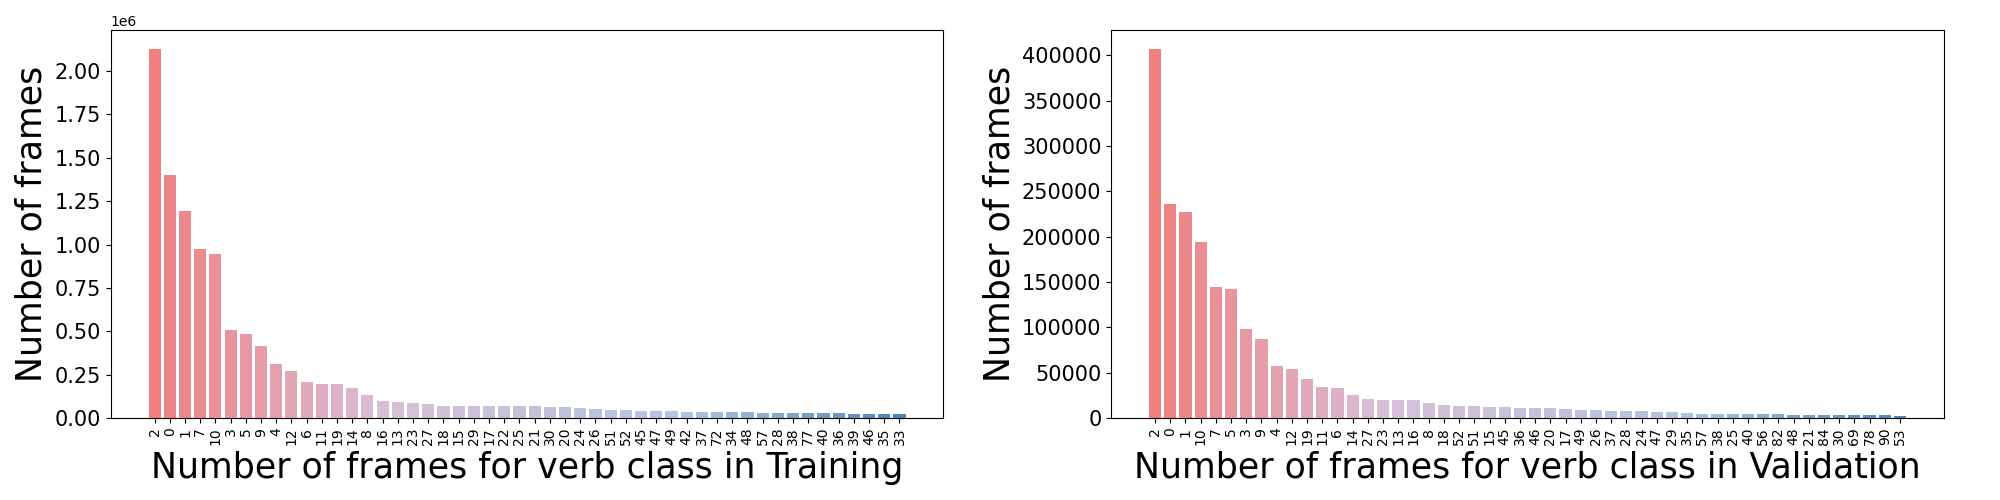
\includegraphics[scale=0.1]{figures/total_frame_word.png}
        % \end{subfigure}
        % \begin{subfigure}[b]{0.475\textwidth}
        %     \centering
        %     \includegraphics[scale=0.3]{figures/avg_number_frames_verb_class_4.png}
        % \end{subfigure}
%         \caption{Histogram of the number of frames in a video}
%         \label{fig:total-frame}
%     \end{minipage}
% \end{figure}

\begin{figure}[htp!]
\begin{minipage}[b]{1\textwidth}
    \centering
    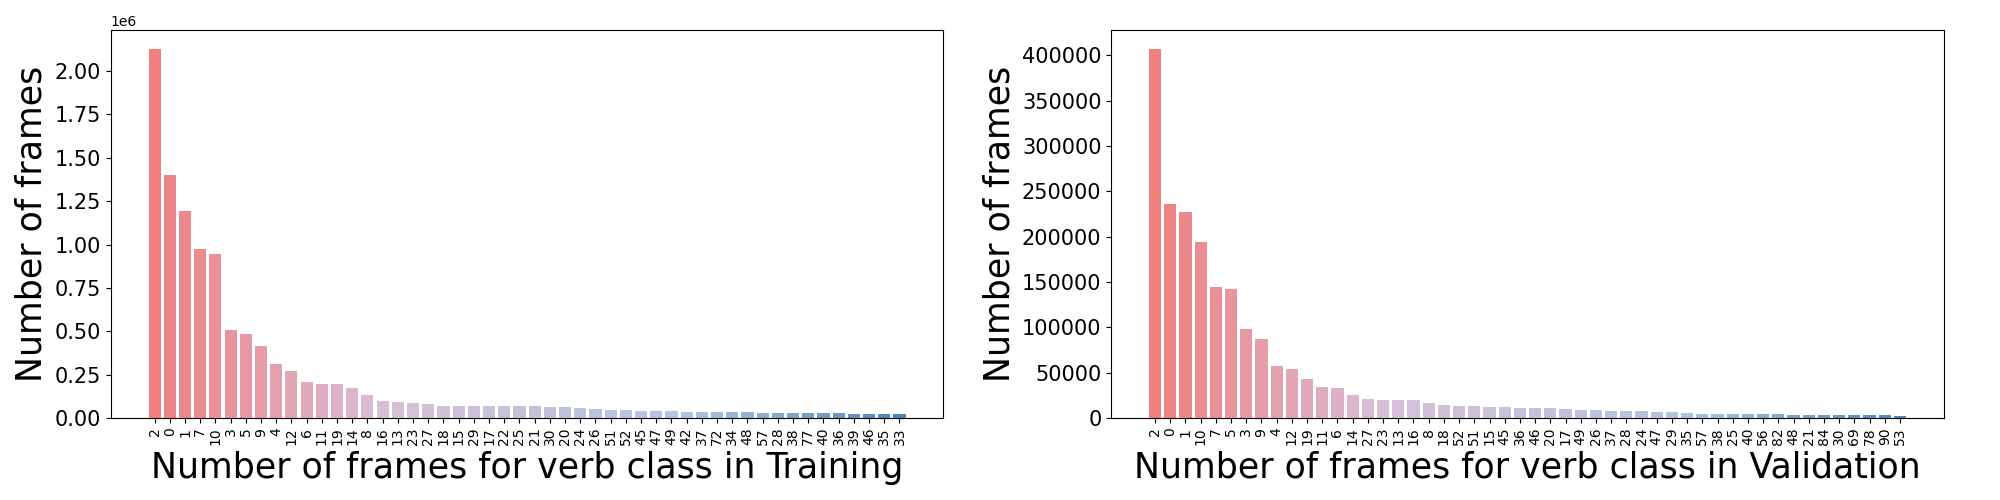
\includegraphics[scale=0.31]{figures/total_frame_word.png}
    \caption{Distribution of number of frames in each video}
    \label{fig:total-frame}
\end{minipage}
\end{figure}

\clearpage

\begin{figure}[t]
    \centering
    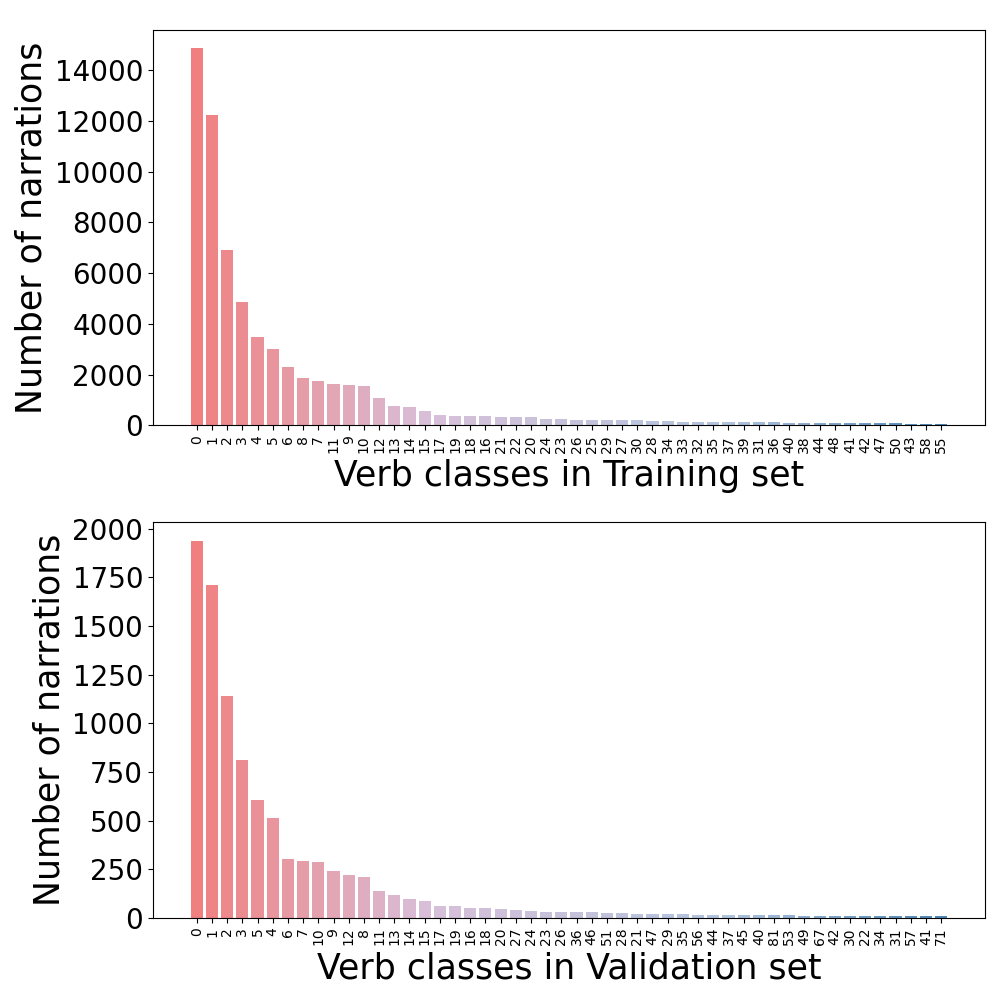
\includegraphics[scale=0.25]{figures/verb_count.png}
    \caption{Frequency distribution of 50 most frequent verb class in training and validation set}
    \label{fig:verb_freq}
\end{figure}

% \subsubsection{Running MSTCN with SlowFast Features} \label{appendix:slowfast}
% We slide 

\begin{figure}[t!]
    % \begin{minipage}[b]{1\textwidth}
        \begin{subfigure}[b]{0.475\textwidth}
            \centering
            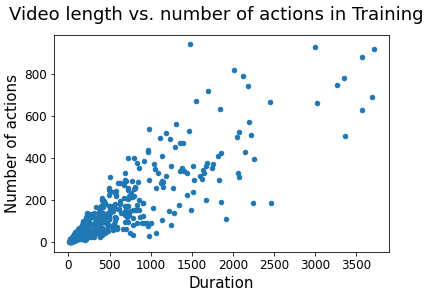
\includegraphics[scale=0.42]{figures/length_vs_actions_Training.png}
        \end{subfigure}\\
        \begin{subfigure}[b]{0.475\textwidth}
            \centering
            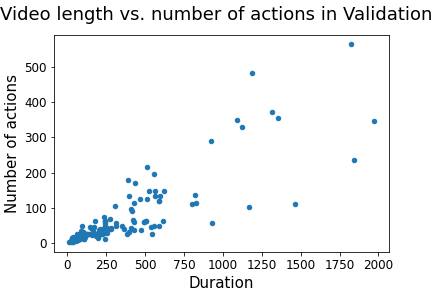
\includegraphics[scale=0.42]{figures/length_vs_actions_Validation.png}
        \end{subfigure}
        \caption{Number of action in each video against video length (in seconds)}
        \label{fig:action-freq-video-length}
    % \end{minipage}
\end{figure}


\subsubsection{Improve Video-Text Matching with Cross-Modal Attention}
The above describes a dual encoder model that independently maps text and video to a joint embedding. It has the advantage in scalability as it can results in efficient evaluation during test time. However, as \newcite{miech2021thinking} points out, it has limited accuracy since the simple dot product is unlikely to capture the complex vision-text interactions. Analogous to how human perform video-text retrieval, one solution is to roughly select a few promising candidates then do fine-grained search for the best candidate by paying more \emph{attention} to visual details. Therefore, we adapt the \emph{Fast} and \emph{Slow} models of \newcite{miech2021thinking} in which the \emph{fast} dual encoder quickly eliminates candidates with low relevance while the \emph{slow} cross-attention model improves retrieval performance with grounding. Given an input segment $\mathbf{v}_i$, we perform retrieval by searching for an action class $\mathbf{c}_j$ such that segment $\mathbf{v}_i$ is most likely to match action class based on the joitnn embedding $\mathbf{c}_j$. Specifically, given segment and action class pair $(\mathbf{v}_i, \mathbf{c}_j)$, we compute their similarity by \[
    h(\mathbf{v}_i, \mathbf{c}_j) = \log (p(\mathbf{c}_j|\phi(\mathbf{v}_i);\theta))
\]
where $\phi(\mathbf{v}_i)$ is extracted feature of segment $\mathbf{v}_i$ and $\theta$ is the parameters of the transformer model. To combine results from dual encoder model and cross-attention model, given input segment $\mathbf{v}_i$ and action class set $\mathcal{C}$ containing $K$ action classes. we first obtain a subset of $m$ action classes $\mathcal{C}_m$ (where $m \ll K$) that have the highest score according to the fast dual encoder model. We then retrieve the final top ranked action class by re-ranking the candidates using the cross attention model:
\[
    \mathbf{y}^*_i=\text{argmax}_{\mathbf{c}_j\in \mathcal{C}_m} h(\mathbf{v}_i, \mathbf{c}_j) + \beta s(\mathbf{v}_i,\mathbf{c}_j)
\]
where $\beta$ is a positive hyper-parameter that weights the output scores of the two models. We output $(\hat{\mathbf{y}}^*_{i,c})$ as the classification probability of frame $i$ as action $c$ based on the similarity score and $(\mathbf{y}^*_i)_{i\in s_i^{3D}}$ as new labels for segment $i,i\in[t]$.


\end{appendices}



\end{document}
